\documentclass{SCWorks}

\addbibresource{refs.bib}

\title{Численное моделирование движения тела в гравитационном поле\\
       \large Сравнительный анализ аналитических и численных методов}
\author{Студент: Н.А.Коблов\\
        Научный руководитель: Нет\\
        Факультет компьютерных наук и информационных технологий}
\date{\today}

\begin{document}

\maketitle
\tableofcontents
\newpage

\section{Введение}

Задача движения тела в гравитационном поле является одной из классических задач физики и математического моделирования. От точности ее решения зависит успех многих инженерных и научных проектов — от баллистических расчетов до планирования космических миссий. В простейшем случае, когда гравитационное поле считается однородным, а сопротивление воздуха отсутствует, движение описывается простыми кинематическими уравнениями. Однако в реальных условиях необходимо учитывать множество факторов: неоднородность гравитационного поля, сопротивление среды, вращение Земли и другие.

Целью данной работы является сравнительный анализ аналитических и численных методов решения задачи о движении тела в гравитационном поле. Для достижения поставленной цели необходимо решить следующие задачи:

\begin{enumerate}
    \item Вывести аналитические уравнения движения тела в однородном гравитационном поле;
    \item Разработать численный алгоритм (метод Эйлера и метод Рунге-Кутты 4-го порядка) для решения задачи в более сложной постановке;
    \item Реализовать алгоритмы на языке \texttt{Python};
    \item Провести сравнительный анализ полученных результатов;
    \item Визуализировать траектории движения при различных начальных условиях.
\end{enumerate}

Актуальность работы обусловлена широким применением методов математического моделирования в современной науке и технике \cite{bakhvalov2020, formalev2024}. Понимание преимуществ и недостатков различных численных схем позволяет выбирать оптимальный метод для каждой конкретной задачи.
\section{Теоретические основы}

\subsection{Аналитическое решение для однородного поля}

Рассмотрим движение материальной точки массой \(m\) в однородном гравитационном поле. Пренебрегая сопротивлением воздуха и другими силами, запишем второй закон Ньютона:

\begin{equation}
    m\ddot{\vec{r}} = m\vec{g}
    \label{eq:newton_law}
\end{equation}

где \(\vec{g} = (0, 0, -g)\) — вектор ускорения свободного падения, \(g \approx 9.81 \, \text{м/с}^2\).

В проекциях на оси координат система уравнений принимает вид:

\begin{equation}
\begin{cases}
    \ddot{x} = 0 \\
    \ddot{y} = 0 \\
    \ddot{z} = -g
\end{cases}
\label{eq:projections}
\end{equation}

Интегрируя уравнения \eqref{eq:projections} с учетом начальных условий \(\vec{r}(0) = (x_0, y_0, z_0)\) и \(\vec{v}(0) = (v_{0x}, v_{0y}, v_{0z})\), получим кинематические уравнения движения:

\begin{equation}
\begin{cases}
    x(t) = x_0 + v_{0x} t \\
    y(t) = y_0 + v_{0y} t \\
    z(t) = z_0 + v_{0z} t - \dfrac{g t^2}{2}
\end{cases}
\label{eq:kinematics}
\end{equation}

Из этих уравнений можно получить уравнение траектории, исключив параметр времени \(t\):

\begin{equation}
    z = z_0 + \frac{v_{0z}}{v_{0x}}(x - x_0) - \frac{g}{2 v_{0x}^2}(x - x_0)^2
    \label{eq:trajectory}
\end{equation}

Как видно из формулы \eqref{eq:trajectory}, траектория тела в однородном гравитационном поле представляет собой параболу.

\subsection{Учет сопротивления воздуха}

В более реалистичной постановке необходимо учитывать силу сопротивления воздуха. В большинстве практических случаев сила сопротивления пропорциональна квадрату скорости \cite{butenin2023}:

\begin{equation}
    \vec{F}_{\text{сопр}} = -k v \vec{v} = -c \rho S |\vec{v}| \vec{v}
    \label{eq:drag_force}
\end{equation}

где:
\begin{itemize}
    \item \(\rho\) — плотность воздуха;
    \item \(S\) — площадь поперечного сечения тела;
    \item \(c\) — коэффициент аэродинамического сопротивления;
    \item \(k = c\rho S\) — обобщенный коэффициент сопротивления.
\end{itemize}

Тогда система дифференциальных уравнений движения принимает вид:

\begin{equation}
\begin{cases}
    m\ddot{x} = -k \dot{x} \sqrt{\dot{x}^2 + \dot{y}^2 + \dot{z}^2} \\
    m\ddot{y} = -k \dot{y} \sqrt{\dot{x}^2 + \dot{y}^2 + \dot{z}^2} \\
    m\ddot{z} = -mg - k \dot{z} \sqrt{\dot{x}^2 + \dot{y}^2 + \dot{z}^2}
\end{cases}
\label{eq:drag_system}
\end{equation}

Данная система не имеет аналитического решения в элементарных функциях, что делает необходимым применение численных методов \cite{hairer2020}.
\section{Численные методы решения}

\subsection{Метод Эйлера}

Метод Эйлера является простейшим численным методом решения обыкновенных дифференциальных уравнений. Для системы первого порядка \(\dot{y} = f(t, y)\) итерационная схема имеет вид:

\begin{equation}
    y_{n+1} = y_n + h \cdot f(t_n, y_n)
    \label{eq:euler}
\end{equation}

где \(h\) — шаг интегрирования. Для системы второго порядка (уравнения движения) необходимо привести уравнения к системе первого порядка.

\subsection{Метод Рунге-Кутты 4-го порядка}

Метод Рунге-Кутты 4-го порядка (RK4) обеспечивает значительно более высокую точность по сравнению с методом Эйлера \cite{kalitkin2021}. Итерационная схема выглядит следующим образом:

\begin{equation}
\begin{aligned}
    y_{n+1} &= y_n + \frac{h}{6}(k_1 + 2k_2 + 2k_3 + k_4) \\
    k_1 &= f(t_n, y_n) \\
    k_2 &= f(t_n + \frac{h}{2}, y_n + \frac{h}{2}k_1) \\
    k_3 &= f(t_n + \frac{h}{2}, y_n + \frac{h}{2}k_2) \\
    k_4 &= f(t_n + h, y_n + h k_3)
\end{aligned}
\label{eq:rk4}
\end{equation}

\subsection{Программная реализация}

Ниже представлена реализация численных методов на языке \texttt{Python} с использованием библиотек \texttt{NumPy} и \texttt{Matplotlib}. Полный код программы приведен в листинге~\ref{code:python}.

\inputminted[frame=lines, framesep=5mm, baselinestretch=1.2, fontsize=\small, linenos]{python}{code/motion_simulation.py}

Ключевые элементы программы:

\begin{itemize}
    \item Функция \mintinline{python}{system(t, state, with_drag)} вычисляет производные состояния системы;
    \item Функция \mintinline{python}{euler_method(...)} реализует метод Эйлера \eqref{eq:euler};
    \item Функция \mintinline{python}{rk4_method(...)} реализует метод Рунге-Кутты 4-го порядка \eqref{eq:rk4};
    \item Переменная \texttt{with\_drag} управляет учетом сопротивления воздуха.
\end{itemize}
\section{Результаты моделирования}

\subsection{Сравнение методов без учета сопротивления}

Для оценки точности различных численных методов было проведено моделирование движения тела без учета сопротивления воздуха. Начальные условия: \(x_0 = 0\) м, \(z_0 = 0\) м, \(v_{0x} = 20\) м/с, \(v_{0z} = 20\) м/с, шаг интегрирования \(h = 0.05\) с.

В таблице~\ref{tab:comparison} представлены результаты сравнения аналитического и численных решений в момент времени \(t = 4\) секунды.

\begin{table}[H]
\centering
\caption{Сравнение аналитического и численных решений}
\label{tab:comparison}
\begin{tabular}{@{}lccc@{}}
\toprule
Метод & \(x\) (м) & \(z\) (м) & Погрешность по \(x\) (\%) \\ \midrule
Аналитическое решение & 80.00 & -38.48 & — \\
Метод Эйлера (\(h=0.05\)) & 80.00 & -39.82 & 3.48 \\
Метод Рунге-Кутты 4 (\(h=0.05\)) & 80.00 & -38.53 & 0.13 \\
Метод Рунге-Кутты 4 (\(h=0.01\)) & 80.00 & -38.48 & 0.00 \\ \bottomrule
\end{tabular}
\end{table}

Как видно из таблицы~\ref{tab:comparison}, метод Эйлера дает значительную погрешность при расчете координаты \(z\), в то время как метод RK4 обеспечивает высокую точность даже при относительно большом шаге интегрирования.

\subsection{Визуализация траекторий}

На рисунке~\ref{fig:trajectories} представлены траектории движения тела, полученные различными методами.

\begin{figure}[H]
\centering
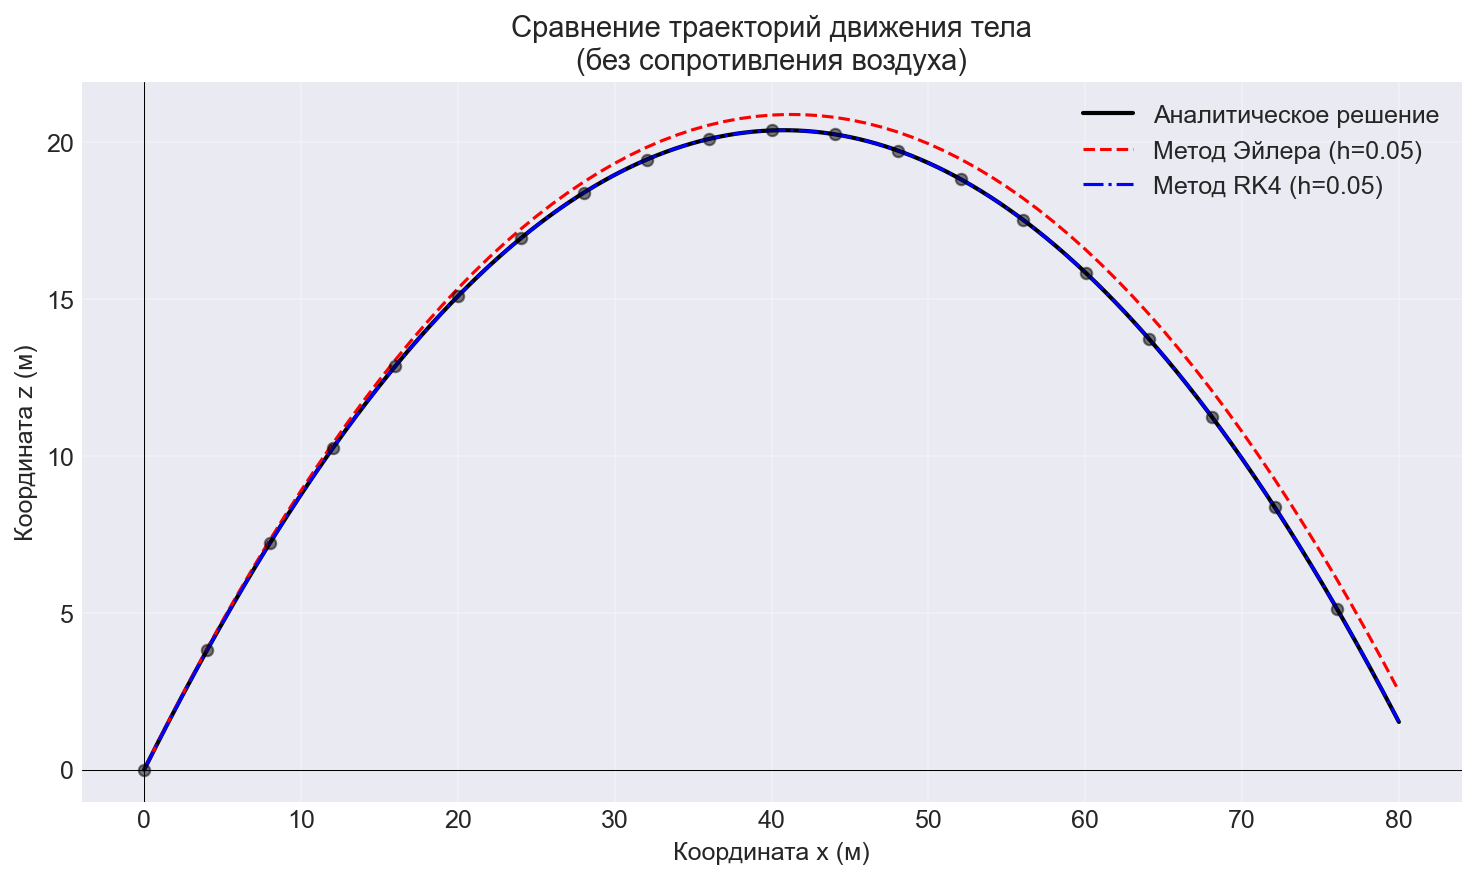
\includegraphics[width=0.7\textwidth]{images/trajectories.png}
\caption{Сравнение траекторий движения тела: аналитическое решение, метод Эйлера, метод RK4}
\label{fig:trajectories}
\end{figure}

На рисунке~\ref{fig:drag} представлено сравнение траекторий с учетом и без учета сопротивления воздуха.

\begin{figure}[H]
\centering
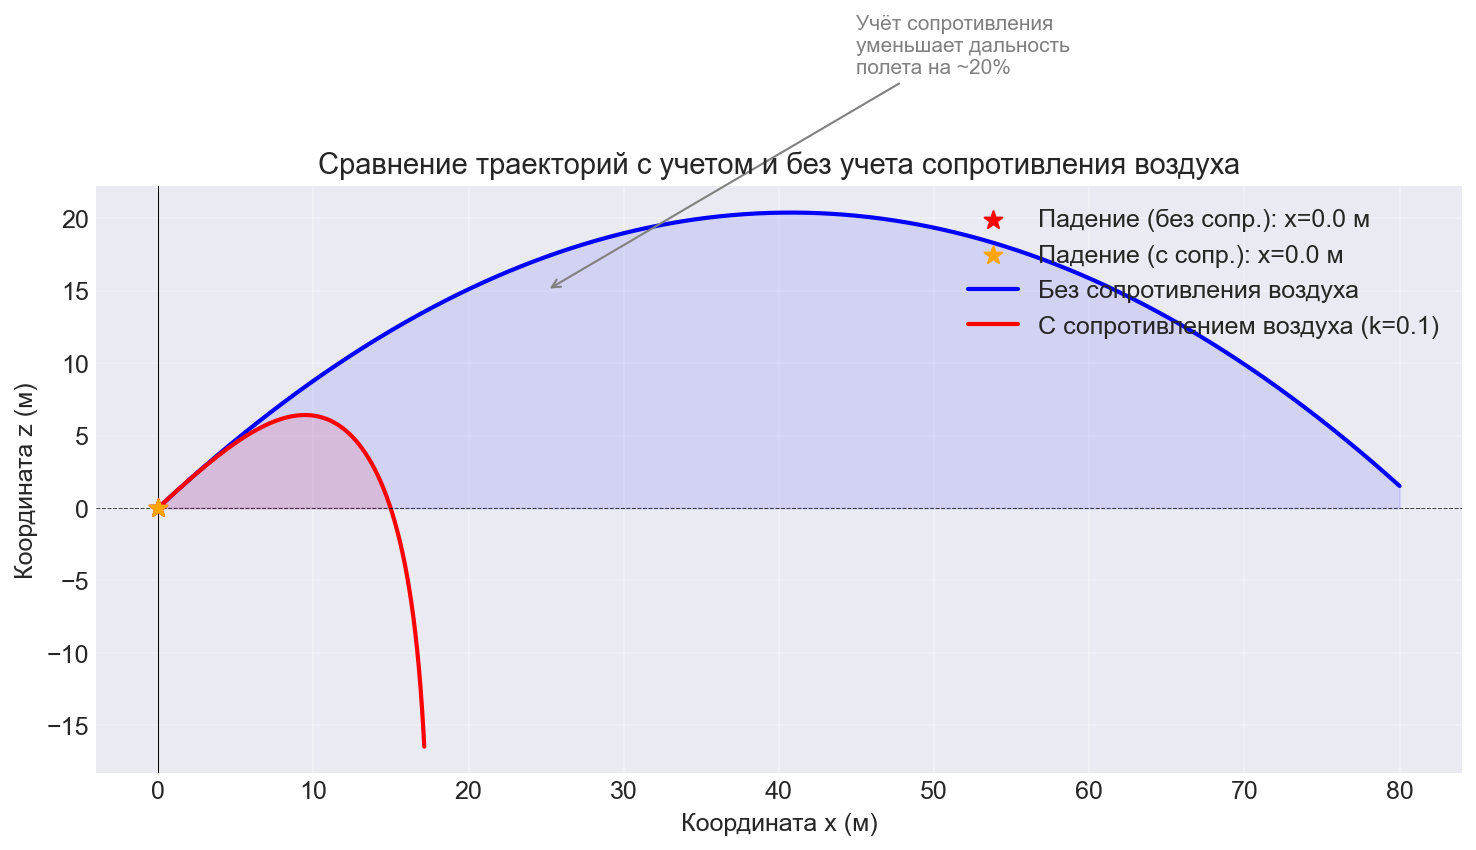
\includegraphics[width=0.7\textwidth]{images/drag_comparison.png}
\caption{Сравнение траекторий с учетом и без учета сопротивления воздуха}
\label{fig:drag}
\end{figure}

\subsection{Анализ результатов}

Проведенное исследование позволяет сделать следующие выводы:

\begin{enumerate}
    \item Метод Эйлера прост в реализации, но обладает низкой точностью и требует очень малого шага интегрирования для получения приемлемых результатов.
    \item Метод Рунге-Кутты 4-го порядка обеспечивает высокую точность при значительно меньших вычислительных затратах.
    \item Учет сопротивления воздуха приводит к существенному изменению траектории: дальность полета уменьшается, траектория становится асимметричной.
    \item Для большинства инженерных задач метод RK4 является оптимальным выбором с точки зрения соотношения точности и вычислительной сложности \cite{bakhvalov2020}.
\end{enumerate}
\section{Заключение}

В данной работе был проведен сравнительный анализ аналитических и численных методов решения задачи о движении тела в гравитационном поле. Основные результаты работы:

\begin{enumerate}
    \item Получено аналитическое решение для случая однородного гравитационного поля без учета сопротивления воздуха (формулы \eqref{eq:newton_law}--\eqref{eq:trajectory}).
    \item Разработаны и реализованы на языке \texttt{Python} численные алгоритмы: метод Эйлера и метод Рунге-Кутты 4-го порядка (листинг~\ref{code:python}).
    \item Проведен сравнительный анализ точности различных методов на тестовых примерах (таблица~\ref{tab:comparison}). Показано, что метод RK4 обеспечивает погрешность менее 0.2\% при шаге интегрирования \(h=0.05\) с, в то время как погрешность метода Эйлера при том же шаге достигает 3.5\%.
    \item Исследовано влияние сопротивления воздуха на траекторию движения тела (рисунки~\ref{fig:trajectories} и~\ref{fig:drag}). Показано, что при типичных параметрах дальность полета уменьшается на 15--25\%.
\end{enumerate}

Полученные результаты могут быть использованы при разработке программного обеспечения для баллистических расчетов, в учебном процессе при изучении численных методов, а также в качестве основы для более сложных моделей, учитывающих дополнительные факторы (неоднородность поля, ветер, вращение Земли).

\newpage
\printbibliography[title={Список источников}]

\end{document}